\documentclass[11pt]{article}
\usepackage{tikz}
\usetikzlibrary{positioning}
\usepackage{amsmath}
\usepackage{geometry}
\geometry{margin=1in}

\title{Lattice Operations in the Imscribing Grammar}
\author{}
\date{}

\begin{document}

\maketitle

\section{Meet, Join, and Tensor}

\subsection{1. Meet (Greatest Lower Bound)}
Takes the minimum in each position.

\begin{center}
\begin{tikzpicture}[node distance=2.5cm]
\node[draw, rectangle, minimum width=3cm] (A) {System A};
\node[draw, rectangle, minimum width=3cm, right=of A] (B) {System B};
\node[draw, rectangle, minimum width=3cm, below=of $(A)!0.5!(B)$] (M) {Meet = A ∧ B};

\draw[->, thick, blue] (A.south) -- (M.north);
\draw[->, thick, blue] (B.south) -- (M.north);
\node[above, blue] at (M.north) {min};
\end{tikzpicture}
\end{center}

\subsection{2. Join (Least Upper Bound)}

\begin{center}
\begin{tikzpicture}[node distance=2.5cm]
\node[draw, rectangle, minimum width=3cm] (A) {System A};
\node[draw, rectangle, minimum width=3cm, right=of A] (B) {System B};
\node[draw, rectangle, minimum width=3cm, below=of $(A)!0.5!(B)$] (J) {Join = A ∨ B};

\draw[->, thick, purple] (A.south) -- (J.north);
\draw[->, thick, purple] (B.south) -- (J.north);
\node[above, purple] at (J.north) {max};
\end{tikzpicture}
\end{center}

\subsection{3. Tensor (Composition with Bottleneck)}

\begin{center}
\begin{tikzpicture}[node distance=3cm]
\node[draw, rectangle, minimum width=3cm] (A) {System A};
\node[draw, rectangle, minimum width=3cm, right=of A] (B) {System B};
\node[draw, rectangle, minimum width=4.5cm, below=2cm of $(A)!0.5!(B)$] (T) {Tensor = A ⊗ B};

\draw[->, thick, teal] (A) -- (T) node[midway, left] {max (most positions)};
\draw[->, thick, red, dashed] (B) -- (T) node[midway, right] {min at Position 4};

\node[below=0.2cm of T, text=red, align=center] {Critical Bottleneck: Position 4 (𐑹 is non-synthesizable)};
\end{tikzpicture}
\end{center}

\section{The Rachis Path}

\begin{center}
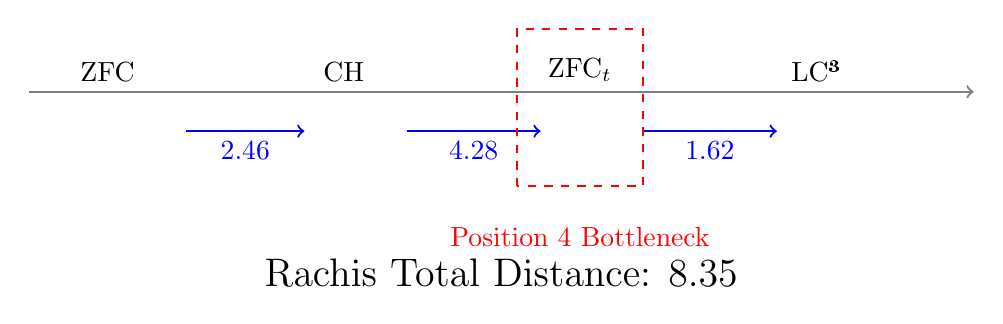
\begin{tikzpicture}
\draw[->, thick, gray] (0,0) -- (12,0);

\node[above] at (1,0) {ZFC};
\node[above] at (4,0) {CH};
\node[above] at (7,0) {ZFC$_t$};
\node[above] at (10,0) {LC³};

\draw[->, blue, thick] (2,-0.5) -- (3.5,-0.5) node[midway, below] {2.46};
\draw[->, blue, thick] (4.8,-0.5) -- (6.5,-0.5) node[midway, below] {4.28};
\draw[->, blue, thick] (7.8,-0.5) -- (9.5,-0.5) node[midway, below] {1.62};

% Bottleneck highlight
\draw[red, thick, dashed] (6.2,-1.2) rectangle (7.8,0.8);
\node[red, below] at (7,-1.6) {Position 4 Bottleneck};

\node[below=2cm] at (6,0) {\Large Rachis Total Distance: 8.35};
\end{tikzpicture}
\end{center}

\section{Tier Distribution}

\begin{center}
\begin{tikzpicture}
\foreach \y/\tier/\pct in {0/O₀/60, 1.5/O₁/8, 3/O₂/18, 4.5/O₂†/6, 6/O_∞/8}{
  \draw[thick] (0,\y) -- (4,\y);
  \node[left] at (-0.3,\y) {\tier};
  \node[right] at (4.3,\y) {\pct\%};
}
\draw[->, thick] (-0.5,0) -- (-0.5,6.5) node[above] {Tier};
\end{tikzpicture}
\end{center}

ZFC starts at O₁. The Rachis skips the entire O₂ tier (18\% of the crystal) and reaches O_∞.

\end{document}